\chapter{Materials and Methods}
\section{Multiple Sequence Alignment}
Multiple sequence alignment (MSA) is a fundamental technique in bioinformatics used to compare and analyze the similarities and differences between multiple biological sequences. These sequences can be DNA, RNA, or protein sequences and can come from various species or different regions of the same genome. By aligning these sequences, it is possible to identify conserved regions that are important for function or evolution, as well as unique features that differentiate the sequences.
% add picture from F. Neiers ?
In this study, we focus on a set of 25 GSTs sequences related to each other through evolution. Each sequence has a different length, making the alignment process especially useful. Through this analysis, we aim to identify regions of conservation and divergence between the sequences (see exemple below). Our first task was to use MSA to predict both the position of the interface of dimerization and the binding site of the set of GST sequence. The stability of the dimer structure is dependent on the interactions at this interface. Therefore, understanding the location and conservation of the dimer interface can provide insights into the stability of the dimer structure and the mechanisms of the biological activity. On the other hand, the binding site is the specific location on the enzyme where a substrate or ligand binds and interacts. The catalytic efficiency of the enzyme is related to the binding site because it determines the specificity and strength of the substrate-enzyme interaction. Therefore, understanding the location and conservation of the binding site is essential for elucidating the function and mechanism of action of the enzyme.\\
\\
\noindent Each cell in the MSA matrix corresponds to a particular amino acid at a particular position in a particular sequence. We refer to the position in the MSA matrix as the MSA index. The MSA index allows us to compare the amino acid residues at each position across all the sequences in the alignment. We focused on highlighting residues that are known to be part of the dimer interface or binding site. By doing so, we can compare these residues across all sequences and identify any conserved or variable regions.

\begin{figure}
	\label{MSA sample}
	\begin{verbatim}
          GSTD1  SPC-RSVIMTAKAVGVELNKKLLNLQAGEHLKPEFLKINPQHTIPTLVDNGFALWESRAI
          GSTE1  SPCVRTVKLTLKVLNLDYEYKEVNLQAGEHLSEEYVKKNPQHTVPMLDDNGTFIWDSHAI
                 SPC R+V +T K + ++   K +NLQAGEHL  E++K NPQHT+P L DNG  +W+S AI
	\end{verbatim}	
	\caption{Sample of a multiple sequence alignment. In such matrix, gaps are represented with the symbol "-". If a residue is conserved, it apears in the last row of the alignment, the residues are in a identical chemical class, thelast raw contains the symbol "+" and eventually, two very different residues are represented by an empty space.}
\end{figure}

\section{AlphaFold}
\noindent As presented in the introduction section, the AlphaFold program allows to make predictions on a protein structure based on its sequence with a prediction comparable with the prediction of X-ray diffraction experiments. In the present work, we used \href{https://colab.research.google.com/github/sokrypton/ColabFold/blob/main/AlphaFold2.ipynb#scrollTo=kOblAo-xetgx}{AlphaFold2} that allows to predict dimeric structures. The program uses 5 different models and evaluate the predictions, we consider only the best predictions.

\section{Anisotropic Network Model}
As seen in the introduction, the AlphaFold program allows for the prediction of protein structures with remarkable accuracy. These structures have the potential to be used in a wide range of applications, including molecular dynamics simulations. In this work, we aim to use AlphaFold-predicted structures as input for the Anisotropic Network Model (ANM) to study protein dynamics. Specifically, we will compare the results obtained from the ANM simulations using AlphaFold structures with those obtained using experimentally determined structures. More precisely, we will use the ANM to predict the thermal B-factors of the studied structures\cite{ANM-COM}, which are important indicators of protein flexibility and stability. The insights gained from this study will contribute to the ongoing efforts to develop computational tools for protein structure analysis and facilitate a deeper understanding of protein dynamics and function. To achieve these goals, it is necessary to provide a detailed description of the ANM and its underlying mathematical principles. The ANM is a widely used method for studying the collective motions and dynamics of proteins based on their structure. It models the protein as a network of connected nodes and springs (representing covalent and non-covalent interactions between them). 

\subsection{Theory}
\noindent Let $\vv{r_i}$ being the position of the node $i$ and $M_i$ it's mass. In the ANM, each node is assumed to be at the bottom of an harmonic potential, since interactions are modeled by connections between nodes, the force matrix is obtained by computing the mass-weighted Hessian matrix
\begin{equation}
	\label{mass-weighted hessian matrix}
	\hat{H}_{ij} = -\gamma\frac{\Gamma_{ij}}{\sqrt{M_iM_j}}\cfrac{\vv{R_{ij}}\vv{R}^T_ {ij}}{R^2_ {ij}}
\end{equation}
where $\gamma$ is the spring constant used to model interactions between nodes, $\vv{R}_{ij} = \vv{R}_j - \vv{R}_i$ and $\Gamma$ is the contact matrix. In the case were $i = j$, the force matrix is computed so that the self interacting term is the response to all the applied forces.
\begin{equation}
	\label{self interacting terms}
	\hat{H}_{ii} = -\sum_{j \ne i}\hat{H}_{ij}
\end{equation}
$\Gamma_{ij}$ is the contact matrix that allow or not two nodes to be interacting with each other. The normal modes and eigenfrequencies are given by the diagonalization of the mass-weighted Hessian matrix.
\begin{equation}
	\label{eigen equation}
	\hat{H}\vv{e}_k = \tilde{\omega}_k^2\vv{e}_k
\end{equation}
First in the equation (\ref{mass-weighted hessian matrix}) $\hat{H}_{ij}$ is a three by three matrix. The ovearall $\hat{H}$ Have a dimention of $d = 3N$ with $N$ the number of considered nodes. The computation time then highly depends on the choosen set of nodes. Second, the masses of the nodes are expressed in g.mol$^{-1}$, expressing $\gamma$ in kcal.mol$^{-1}$.\AA$^{-2}$, the eigenvalues $\tilde{\omega}_k^2$ are expressed in kcal.g$^{-1}$.\AA$^{-2}$ which is directly proportional to a squared frequency $\omega^2 = 4.184 \times 10^{26}$ s$^{-2}$. Thermal B-factors are extracted from X-ray diffraction experiment that are directly proportional to the mean squared fluctuations $\sigma^2(\vv{R}_i)$ computed from ANM
\begin{equation}
	\label{thermal B-factors}
	\sigma^2(\vv{R}_i) = k_BT\sum_k\frac{1}{\tilde{\omega}_k^2} \cfrac{\vert\vv{e}_{k, i}\vert^2}{M_i}
\end{equation}
where $\vv{e}_{k, i}$ contains the elements of $\vv{e}_k$ related to the node $i$. $\sigma^2(\vv{R}_i)$ is expressed in m$^2$ but will always be converted in $\AA^2$ because of conventions and usual order of magnitude.\\
\noindent Ever since the beginning, we were talking in a very abstract way about "nodes". In this work, we did consider the amino-acid's center of mass (COM). When available, we compared the predicted values of B-factors with X-ray based measurement in term of pearson correlation.
\begin{equation}
	\label{pearsonr}
	\mathcal{R} = \cfrac{\displaystyle\sum_i (\beta_i - <\beta>_i)(B_i - <B>_i)}{\sqrt{\displaystyle\sum_i(\beta_i - <\beta>_i)^2}\sqrt{\displaystyle\sum_j(B_j - <B>_j)^2}}
\end{equation}
The values of $\mathcal{R}$ are between $-1$ and $1$ and gives the linear correlation between predicted and measured B-factors. A coefficient of $1$ is associated to a perfect correlation wherease a coefficient of $0$ means that there is basically no links between prediction and experiment. Eventually, a negative value of $\mathcal{R}$ means that there is a correlation with opposite sign and would be interpreted as a result even worst than no correlation. Note that we need to consider the same ensemble of points for $\beta_i$ and $B_i$.\\
\noindent The thermal fluctuation of the nodes is not the only informations one can get from normal modes, indeed fluctuations of the $\vv{R}_{ij}$ vector can also be an interesting metric to analyse as it represents the relative motion of nodes within a given mode. 
\begin{equation}
	\label{metric dij}
	\sigma^2 (\vv{R}_{ij}) = k_BT\sum_k \frac{1}{\omega_k^2}\left( \frac{\vv{e}_{k, j}}{\sqrt{M_j}} - \frac{\vv{e}_{k, i}}{\sqrt{M_i}} \right)^2
\end{equation}
Such metric is especially interesting to study as it provide insights about the fluctuations of a mode with respect to another and allow to identify pairs of nodes involved in specific functional modes.
\subsection{Parametrization}
In the Anisortopic network model as presented above, we consider two parameters namely the contact matrix $\Gamma_{ij}$ and the spring constant $\gamma$. In order to get predictions that are physically relevant, it is necessary to compute the good parameters. Let us first consider the contact matrix. Given two nodes $i$ and $j$, we will consider $\Gamma_{ij} = 1$ if the distance $\vert\vv{R}_{ij}\vert$ is smaller than the cut-off $R_c$. It is then necessary to find a good numerical value for $R_c$. We know that for high distances, the interactions between the nodes are supposed to be small if not nulls. To add this kind of interactions, we look for $R_c$ as small as possible. We also know that the eigenvalues are associated to frequencies for the collectives modes. The six firsts modes should be global transations and rotations with a null frequency associated. In the case where $R_c$ is too small, some other modes will have null eigenfrequencies with no physical justifications. $R_c$ is then the smallest value that gives exactly $6$ null eigenvalues for the Hessian. Eventually, in the equation (\ref{mass-weighted hessian matrix}) $\gamma$ is a constant, it means that $\tilde{\omega}_k^2 \propto \gamma$. From the equation (\ref{thermal B-factors}), one can show that $\beta_i$ is inversly proportional to $\gamma$ which is just a scaling factor. It can then be computed from comparitions with experimental measurments of thermal B-factors using least squared methods.

\begin{figure}[h!]
	\label{Rc param}
	\begin{minipage}{.48\linewidth}
		\textbf{A}\\
		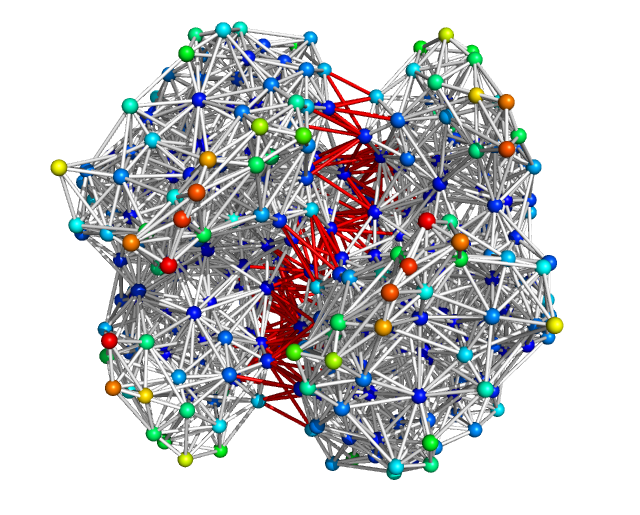
\includegraphics[width = .99\linewidth]{figures/GSTD1_ElasticNetwork.png}
	\end{minipage}	
	\begin{minipage}{.48\linewidth}
		\textbf{B}\\
		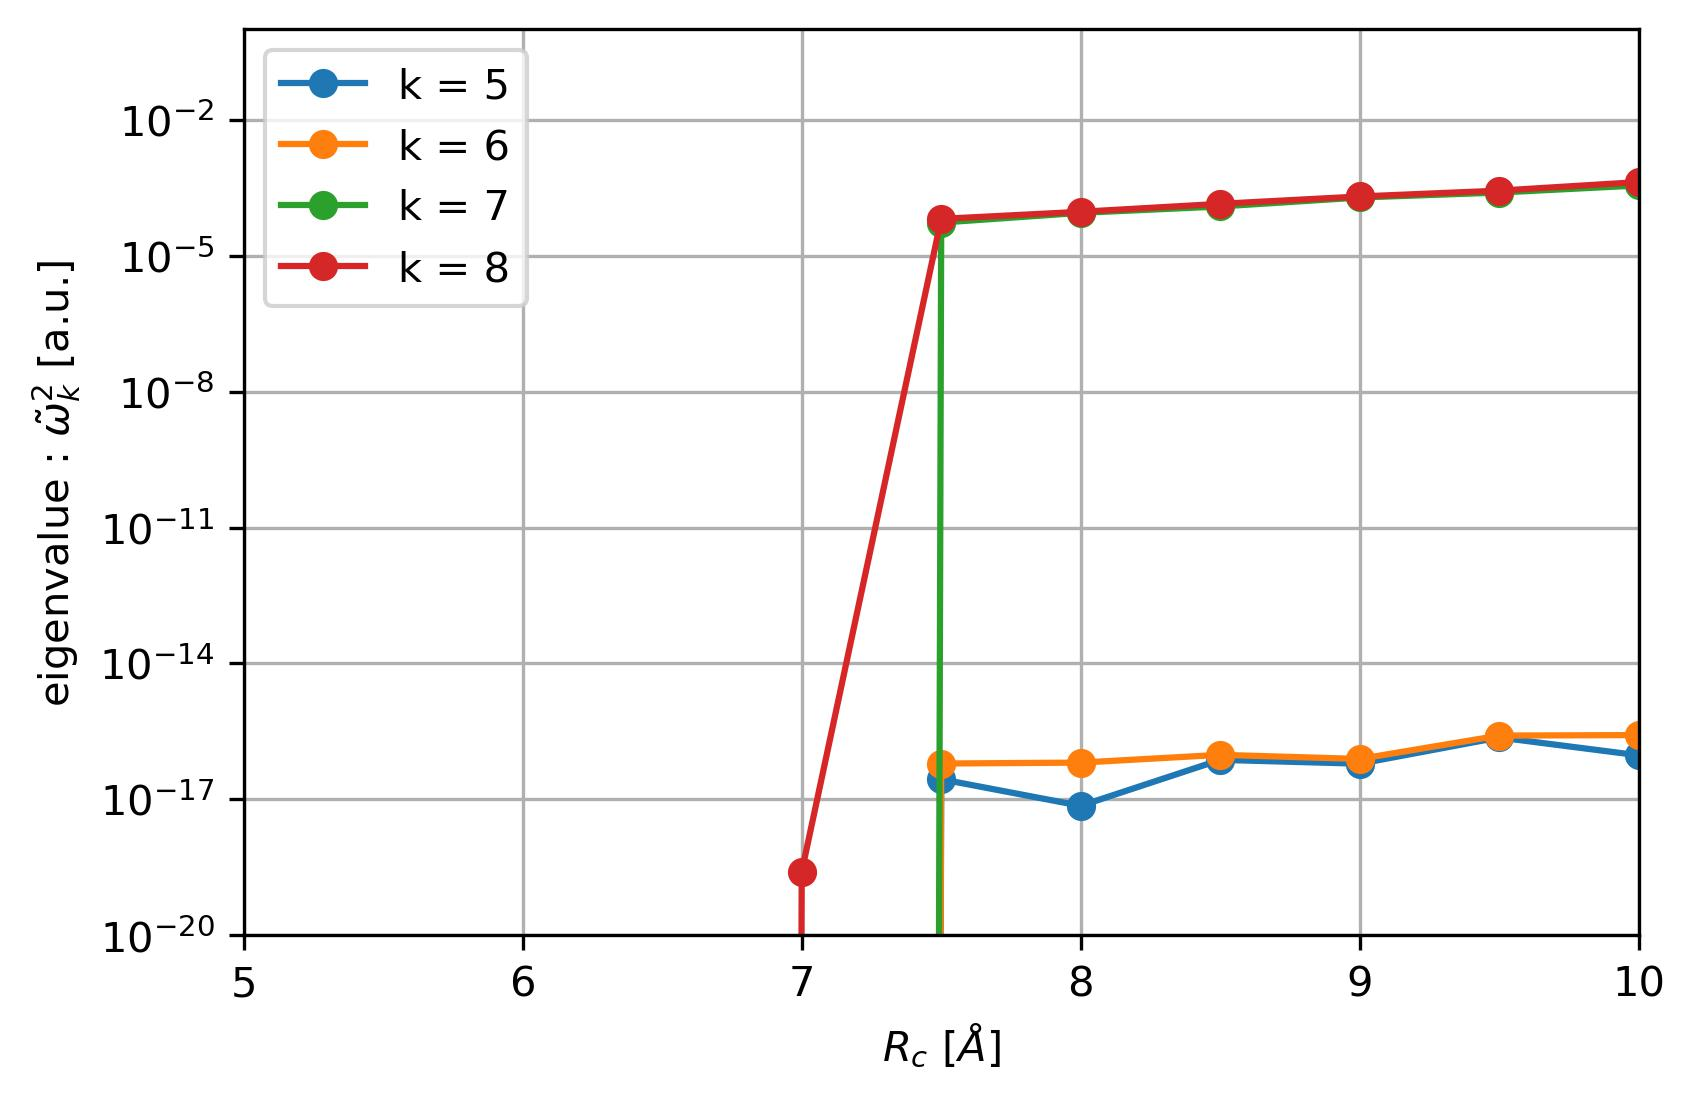
\includegraphics[width = .99\linewidth]{figures/GSTD1_ANM-COM_Rc_param.jpg}\\[.5cm]
	\end{minipage}	
	\caption{Coarse grained representation \& cut-off parametrisation of GSTD1 structure}	
\end{figure}

\noindent In the figure \ref{Rc param}, it is clearly visible that for $R_c = 7.5\AA$, the eigenvalues for $k \ge 6$ are no longer nulls. It is then convenient to use this value of cut-off for this structure. Note that later, such computations will be performed for all 25 structures in order to have a correct representation of the structures' topology. Those eigenvalues are computed for $\gamma = 1$ kcal.mol$^{-1}$.\AA$^{-2}$, but as we have seen before, $\tilde{\omega}_k^2 \propto \gamma$. It is now time to compute the thermal B-factors to be able to compute the optimal $\gamma$ value.

%\section{Molecular Dynamics}
%Molecular dynamics (MD) has emerged as a powerful computational tool for simulating molecular systems with exceptional precision. By numerically integrating the equations of motion for atoms and molecules, MD provides detailed information about the dynamic behavior and interactions within these systems. With its ability to capture the atomic-level motion and thermodynamics, MD offers insights into the structural changes, energetics, and properties of molecules under various conditions. Compared with ANM, MD stands out for its superior precision in capturing the dynamic behavior of molecular systems. For the purpose of this work, the amount of system to be studied is far too big ($25$ structures $\times 3$ states in the catalytic cycle) and cannot be considered as an option. But considering it's accuracy, one can consider a sample of GSTs that will be simulated via MD.\\
%MD consider interactions between atoms in a large variety of form. First, non-bonded interactions are considered with a lehnard-jones potential and electrostatic interactions.
%\begin{equation}
%	\label{non-bonded}
%	V_{\text{non-bonded}}(\vv{r}_i) = \sum_j 4\epsilon_{ij}\left[ \left( \frac{\sigma_{ij}}{R_{ij}} \right)^{12} - \left( \frac{\sigma_{ij}}{R_{ij}} \right)^{6} \right] + \sum_j\cfrac{q_iq_j}{4\pi\epsilon_0R_{ij}}
%\end{equation}
%Interactions between bonded atoms are also described by the following.
%\begin{equation}
%	\label{bonded}
%	V_{\text{bonded}}(\vv{r}_i) = \sum_{\text{bonds}} K_l(l - l_0)^2 + \sum_{\text{angles}} K_\theta(\theta - \theta_0)^2 + \sum_{\text{tortions}} K_\varphi [1 + \cos (n\varphi + \delta)]
%\end{equation}
%The ensemble of parameters for those interactions are optimized and used by MD algorithms by the so called force fields. Since the potential consider interactions between all the atoms of the system, this kind of simulation is called All Atoms MD, in opposition to coarse grained MD that we wont discuss here. Finally forces of interactions are obtained taking the gradient of the potential and the simulation is achieved by integration of the Newton's equation :
%\begin{equation}
%	\label{Newton}
%	m\frac{d^2\vv{r}_i}{dt^2} = -\vv{\nabla}V(\vv{r}_i)
%\end{equation}
%From the time serie obtained, one can compute the associated Thermal B-Factors as mean squared fluctuations of the atom's position.
%\begin{equation}
%	\label{MD thermal B-factors}
%	\beta_i = \frac{8\pi^2}{3}\left(\left< \vv{R}_i^2 \right> - \left< \vv{R}_i \right>^2\right)
%\end{equation}
%Comparisons between such factors computed from MD and from ANM gives again extra informations about the precision of the considered models.